\setcounter{page}{1}

\section{Fondements}
\subsection{Historique}
Le C est un langage de programmation apparu dans les années 70, dérivant directement du langage B, et inventé par 	Dennis Ritchie et Kenneth Thompson. C'est un langage impératif, procédural et bas niveau. En conséquence de quoi, il permet d'ériger des séquences d'instructions qui offrent, entre autre par le biai des pointeurs et des accès aux primitives du systèmes, une manipulation ample mais périlleuse du hardware.

Notons qu'une grande partie des processeurs sont de natures impératives ; subséquemment, il est naturel que les langages de programmations \_ qui visent en outre à simplifier l'interaction homme/machine et le contrôle de celle-ci \_ se rapprochent d'un tel paradigme.
%%%%%%%%%%%%%%%%%%%%%%%%%%%%%%%%%%%%%%%%%
\subsection{La compilation}
Le C est un langage compilé. Le code est préalablement édité dans un \textit{fichier source} dont l'extension est \textit{.c} avant d'être traduit en langage machine (assembleur) par le compilateur. On décrit ci-dessous les différentes étapes de la compilation.
\subsubsection{Pré-traitement}
Lors de cette phase de pré-traitrement, le pré-processeur procède en une mise aux normes textuelles du fichier source.
\begin{itemize}
    \flch Remplacement des \hyperlink{https://learn.microsoft.com/fr-fr/cpp/c-language/trigraphs?view=msvc-170}{\textit{tri-graphes}}
    \flch Raccordement des lignes qui forment une unité logique
    \flch Retrait des commentaires
    \flch Expansion des macros et exécution des directives spécifiques (inclusion d'autres fichiers...)
\end{itemize}
\subsubsection{Analyse lexicale}
Aussi appellée \textit{tokenization}, elle procède en une conversion de chaînes de caractère en symboles appelés \textit{token}. 
\subsubsubsection{Unités lexicales}
La convention syntaxique ANSI exhibe les \textit{jetons/ unités lexicales/ lexèmes/ tokens} suivant:\\
\begin{table}[h]
    \centering
    \begin{tabular}{p{2.5cm}p{3cm}}
        \textbf{Token} & \textbf{Exemple}\\
        mot-clé & \mintinline{c}{if extern char}\\
        identifiant & \mintinline{c}{mafonction x y}\\
        constante & \mintinline{c}{0 15.3 1e-4 'c' "coucou"}\\
        chaîne & \mintinline{c}{"coucou" true}\\
        opérateur & \mintinline{c}{*+-}\\
        ponctuation & \mintinline{c}{();}\\
    \end{tabular}
    \caption{Unités lexicales du C}
    \label{tab:tokentab}
\end{table}
\begin{rem}{0}
    Toutes ces composantes lexicales sont détaillées par la suite.
\end{rem}
\newpage
\subsubsubsection{Processus}
Afin de procéder à l'analyse lexicale, et d'exhiber les tokens appartenant au langage de programmation, il est judicieux de se munir d'automates. Ce faisant, un automate fini permet d'opérer un \textbf{balayage} du code source afin de déterminer chacun des lexèmes qui le compose en leur adjoignant leur type.\\[0.5cm]
\noindent
\textbf{Exemple}\\
De façon concrète, nous pouvons concevoir un automate qui reconnaît les entiers générés par une expression rationnelle ($['0'-'9']^{*}$)
\begin{figure}[h]
    \centering
    \includegraphics[scale=0.8]{poly005.png}
    \caption{Automate reconnaissant les entiers \cite{Maranget}}
    \label{fig:aut1}
\end{figure}\\
Il faut ainsi imaginer qu'il en est de même pour le reste du langage.\\[0.5cm]
Ensuite, l'\textbf{évaluation} convertit chaque lexème en une valeur. C'est aussi au cours de cette opération que les \textit{espaces blancs} (à savoir les tabulations, les caractères espaces, les sauts de ligne...) sont supprimés.\\

\noindent
\textbf{Exemple}\\
Considérons l'instruction \mintinline{c}{sum = 2 + 3;}. L'analyse lexicale produit une liste de lexèmes munis de leurs types, de telle sorte à être conforme à la \textbf{grammaires du langage} ainsi qu'à ses \textbf{regles de productions}.
\begin{minted}{ocaml}
    [(identifiant, sum), (opérateur d'affectation, =), (entier littéral, 2), (operator, +), (entier littéral, 3), (fin de déclaration, ;)]
\end{minted}
\subsubsection{Analyse syntaxique}
La précédente analyse lexicale nous a permis de mettre en exergue un flux de lexèmes. Lors de l'analyse syntaxique ou grammaticale, on établit un arbre connexe acyclique qui décrit l'intrication syntaxique de notre code source en fonction de la grammaire (dite algébrique ou non contextuelle) du langage.\\[0.5cm]
\noindent
\textbf{Exemple}\\
Considérons l'expression $\phi=(x+1)*(3*y+2)$. L'arbre de syntaxe abstraite représentant $\phi$ est le suivant:
\begin{figure}[h]
    \centering
    \includegraphics[scale=0.7]{arbsyntax.png}
    \caption{Arbre de syntaxe \cite{levy}}
    \label{fig:arbsyntax}
\end{figure}
\newpage
\subsubsection{Suite et fin...}
Suite à l'analyse sémantique, on obtient un code intermédiaire qu'il convient de transformer en code assembleur (langage machine). S'en suit un processus d'optimisation, d'allocation mémoire et d'édition des liens afin de produire, enfin, un fichier exécutable.

\begin{rem}{0.5}
    Le détail du processus de compilation est plus riche et plus complexe que ce que cours mentionne. On se contente de ne donner que quelques éléments notionnels sur les grandes étapes du processus. Un cours complet de compilation repose sur la théorie des langages, la Sémantique Opérationnelle Structurelle, une connaissance du hardware... Se référer à la bibliographie pour plus de détails.
\end{rem}
\subsubsection{Le compilateur GCC}
Afin de compiler notre fichier source sous UNIX, on se munira du compilateur GCC développé par le projet GNU. L'appel au compilateur suit la syntaxe suivante:
\begin{minted}{bash}
gcc [options] fichier.c [-llibrairies]
\end{minted}
\subsubsubsection{Options}
\vspace*{-0.5cm}
\begin{itemize}
    \flch \mintinline{bash}{-c} : Stoppe la compilation au stade du fichier objet. 
    \flch \mintinline{bash}{-o nom-de-fichier} : Renommage du fichier produit. Par défaut, le exécutable fichier
s’appelle a.out.
    \flch \mintinline{bash}{-Wall} : Affiche l'ensemble des messages d'erreur.
    \flch \mintinline{bash}{-O, -O1, -O2, -O3} : options d’optimisations, de la plus faible à la plus importante.
\end{itemize}
\subsubsubsection{En pratique}
Admettons que nous ayons codé notre programme dans le fichier \textit{mon\_Prog.c}.
\begin{minted}{bash}
    gcc mon_Prog.c -o exe       #Permet de générer un executable "exe"
    ./exe                       #Permet de lancer l'exécutable
\end{minted}

\begin{rem}{0.5}
    On se référera au chapitre sur le paradigme de la programmation modulaire pour une pratique de compilation plus évoluée.
\end{rem}

%%%%%%%%%%%%%%%%%%%%%%%%%%%%%%%%%%%%%%%%%

\subsection{Les expressions}
Une expression est constituée des lexèmes vus précédemment.
\subsubsection{Identificateur}
\label{ident}
Une notation d'affectation peut commencer par:
    \begin{itemize}
        \item Une lettre (min,MAJ)
        \item Un underscore (\_)
    \end{itemize}
    et peut contenir des entiers.\\
\warning ~ Elle ne peut pas commencer par un entier. Ex: "5Id\_Min" n'est pas valide.
%%%%%%%%%%%%%%%%%%%%%%%%%%%%%%%%%%%%%%%%%



\subsection{Types de bases}
Le C est un langage à typage statique. En conséquence de quoi, il faut faire figurer le type de chacun des objets ; de la sorte, lors de la compilation, un espace mémoire suffisant est alloué à chaque variable.
\subsubsection{Type entier}
Les valeur entières sont caractérisées par le mot-clé \mintinline{c}{int}. Toutefois, il est possible de spécifier l'amplitude numérique et le signe de la valeur entière à stocker. Pour ce faire, il faut faire précéder \mintinline{c}{int} par \mintinline{c}{short / long / long long}, et éventuellement de \mintinline{c}{signed / unsigned} si l'entier est positif ou-bien de signe quelconque.


\begin{table}[h]
    \centering
    \begin{tabular}{c|ccc}
         & Encodage (bits) & Valeur minimal & Valeur maximale\\
         \hline
        char & 8 &  -127 & 127 \\
        short & 16 & -32 767 & 32 767\\
        int & 32 & -32 767 & 32 767\\
        unsigned int & 32 & 0 & 32 767\\
        long & 32 & -2 147 483 647 & 2 147 483 647\\
        long long  & 64 & -$2^{64}$ & $2^{64}-1$ \\
    \end{tabular}
    \caption{Domaines \& encodages du type \mintinline{c}{int}}
    \label{tab:domint}
\end{table}

\subsubsection{Type float}
Les valeurs réelles sont typées par le mot-clé \mintinline{c}{float}. Elles sont représentées syntaxiquement comme suit: \mintinline{c}{float x=15.8;}
\begin{table}[h]
    \centering
    \begin{tabular}{c|ccc}
         & Encodage (bits) & Valeur minimal & Valeur maximale\\
         \hline
        float & 32 & 0 & 32 767\\
        double & 64 & -2 147 483 647 & 2 147 483 647\\
        long double  & 128 & -$2^{64}$ & $2^{64}-1$ \\
    \end{tabular}
    \caption{Domaines \& encodages du type \mintinline{c}{int}}
    \label{tab:domfloat}
\end{table}

Sur un ordinateur, on utilise les nombres à virgule flottante de la
forme $x = s * m * b^e$ où b est la base ; s $\in {-1,+1}$ est le signe ;
la mantisse m, ou significande, précise les chiffres significatifs ;
l’exposant e donne l’ordre de grandeur. Pour plus de détails, se référer à l'annexe.

\subsubsection{Type bool}
Il n'existe pas de type booléen à proprement parlé en C. En effet, on assimile la valeur \textbf{vrai} à 1 et \textbf{faux} à 0. De fait, il est possible de manipuler des valeurs booléennes en opérant sur $\{0;1\}$ ou-bien en définissant des \textit{macros}. Cette notion de macros n'ayant pas encore été introduite ; il sera préférable (et équivalent) d'utiliser la librairie \mintinline{c}{stdbool.h} qui définit les constantes \mintinline{c}{true false} ainsi que type \mintinline{c}{bool}.

\begin{rem}{0.5}
    On se référera à la sous-section \nameref{cp} page \pageref{cp} (Annexe) concernant les rappels en \textbf{logique mathématiques}.
\end{rem}
\subsubsection{Type caractère}
Le type caractère est désigné par le mot-clé \mintinline{c}{char}, quoique les caractères puissent être assimilés à des entiers selon leur code ASCII.\\
Les \mintinline{c}{char} sont codés sur un octet (8 bits) et tolèrent les opérations arithmétiques propres aux entiers. De plus, les objets de ce type sont explicitement représentés entre  guillemets simples: \mintinline{c}{'a'}
\begin{minted}{c}
    char caractere='c';
    printf("Le caractère suivant dans la table ASCII est: %c",caractère+1);
    // Affiche 'd'
\end{minted}
\begin{table}[h]
    
    \begin{minipage}{0.5\textwidth}
    \centering
        \begin{tabular}{|c|c||c|c||c|c|}
        \hline
         & dec &   & dec &  & dec\\
         \hline \hline
          & 32 & @ &  64& ' & 96\\
         \hline
         !& 33 & A &  65& a & 97\\
         \hline
         "& 34 & B &  66& b & 98\\
         \hline
         \#& 35 & C & 67 & c & 99\\
         \hline
         \$& 36 & D &  68& d & 100\\
         \hline
         \%& 37 &  E&  69& e & 101\\
         \hline
         \& & 38 &  F&  70& f & 102\\
         \hline
         `& 39 & G &  71& g & 103\\
         \hline
         (& 40 & H & 72 & h & 104\\
         \hline
         )& 41 &  I& 73 & i & 105\\
         \hline
         *& 42 &  J&  74& j & 106\\
         \hline
         +& 43 &  K&  75& k & 107\\
         \hline
         ,& 44 &  L&  76& l & 108\\
         \hline
         -& 45 &  M&77  & m & 109\\
         \hline
         .& 46 &  N&  78& n & 110\\
         \hline
         /& 47 &  O&  79& o & 111\\
         \hline
    \end{tabular}
    \end{minipage}
    \begin{minipage}{0.5\textwidth}
    \centering
        \begin{tabular}{|c|c||c|c||c|c|}
        \hline
         & dec &   & dec &  & dec\\
         \hline \hline
         0& 48 &  P&  80& p & 112\\
         \hline
         1& 49 &  Q&  81& q & 113\\
         \hline
         2& 50 &  R&  82& r & 114\\
         \hline
         3& 51 &  S&83  & s & 115\\
         \hline
         4& 52 &  T&  84& t & 116\\
         \hline
         5& 53 &  U& 85 & u & 117\\
         \hline
         6& 54 &  V&  86& v & 118\\
         \hline
         
         7& 55 &  W&  87& w & 119\\
         \hline
         8& 56 &  X& 88 & x & 120\\
         \hline
         9& 57 &  Y&  89& y & 121\\
         \hline
         :& 58 &  Z&  90& z & 122\\
         \hline
         ;& 59 &  [ &  91& \{ & 123\\
         \hline
         <& 60 & \ & 92 & | & 124\\
         \hline
        = & 61 & ] & 93 & \} & 125\\
         \hline
        > & 62 &  ĉ & 94 & - & 126\\
         \hline
        ? & 63 &  \_ & 95 &\footnotesize{DEL} & 127\\
         \hline
    \end{tabular}
    \end{minipage}
    
    \caption{Code ASCII}
    \label{tab:ascii}
\end{table}
\subsubsubsection{Manipulation des caractères \textcolor{red}{A faire}}
%Fonction: ishupper islower, isalpha
%somme de caractères 'a'+'b'=? -base 26
\subsubsection{Type chaîne de caractère}
Les chaînes de caractères sont de type \mintinline{c}{char*}. Lorsqu'elles sont définies explicicement, elles sont implémentées entre guillemets doubles: \mintinline{c}{"ainsi"}.
\begin{rem}{0.5}
    En réalité, les chaînes de caractères sont des tableaux de caractères. On se référera à la sous-section XX page XX pour plus de détails sur les chaînes de caractères.
\end{rem}
\newpage
\subsection{Les opérateurs}
\subsubsection{Opérateur d'affectation}
L'affectation d'une expression \mintinline{c}{e} à variable \mintinline{c}{x} de type \mintinline{c}{t} s'effectue avec l'opérateur \mintinline{c}{=}.\\
De plus, lors de la compilation de l'instruction:
\begin{minted}{c}
    t1 x = e;
\end{minted}
l'expression \mintinline{c}{e} est convertie dans le type de la variable, en l'occurrence \mintinline{c}{t1} ici. On appelle celà le \textit{transtypage} (\textit{cast} en anglais).\\[0.5cm]
Afin de présenter les différents opérateurs, on utilisera la notation suivante: 

\begin{table}[h]
    \centering
    \begin{tabular}{cc}
       $\bullet|^n_{F}$ & où $\left\lbrace \begin{array}{ll}
n & \text{est l'arité de l'opérateur}\\
S & \text{est le type du résultat}\\
\end{array}\right.
$\\
    \end{tabular}
    \label{tab:notation}
\end{table}
\subsubsection{Opérateurs arithmétiques}
Le type de retour est
\mintinline{c}{type}=$\left\lbrace \begin{array}{ll}
\mintinline{c}{int} & \text{si les opérandes sont de types \mintinline{c}{int}}\\
\mintinline{c}{float} & \text{si tout ou partie des opérandes sont de type \mintinline{c}{float}}\\
\end{array}\right.
$
\begin{table}[h]
    \centering
    \begin{tabular}{cccccc}
        Addition & Soustraction & Multiplication & Division entière & Modulo & Division réelle\\
        $+\big|^{~2}_{\scriptsize\mintinline{c}{type}}$ & 
        $- \big|^{~2}_{\scriptsize\mintinline{c}{type}}$ & 
        $* \big|^{~2}_{\scriptsize\mintinline{c}{type}}$ &
        $/\,\big|^{~2}_{\scriptsize\mintinline{c}{type}}$ & 
        $\% \big|^{~2}_{\scriptsize\mintinline{c}{int}}$ & 
        $/ \big|^{~2}_{\scriptsize\mintinline{c}{float}}$\\
    \end{tabular}
    
    \label{tab:my_label}
\end{table}
\subsubsection{Opérateurs de comparaison}
\begin{table}[h]
    \centering
    \begin{tabular}{cccccc}
        $<\big|^{~2}_{\scriptsize\mintinline{c}{bool}}$ & 
        $<= \big|^{~2}_{\scriptsize\mintinline{c}{bool}}$ & 
        $> \big|^{~2}_{\scriptsize\mintinline{c}{bool}}$ &
        $>=\,\big|^{~2}_{\scriptsize\mintinline{c}{bool}}$ & 
        $!= \big|^{~2}_{\scriptsize\mintinline{c}{bool}}$ & 
        $== \big|^{~2}_{\scriptsize\mintinline{c}{bool}}$\\
    \end{tabular}
    
    \label{tab:opcomp}
\end{table}
\begin{code}
\dangersign[2.5ex] \,\textbf{Test d'égalité sur les \mintinline{c}{float}}\\
On ne réalise pas de test d'égalité sur les flotant en utilisant l'opérateur \mintinline{c}{==}\\
Lorsque l'on souhaite tester l'égalité entre deux réels, il faut réaliser un encadrement à $\varepsilon$ près, $\varepsilon$ étant la précision souhaitée. 
\end{code}
\begin{rem}{0.5}
    L'oubli du double égal, au profit d'un = est l'une des principales source d'erreur de compilation.
\end{rem}
\subsubsection{Opérateurs booléens}
\begin{table}[h!]
    \centering
    \begin{tabular}{ccc}
        $\&\&\big|^{~2}_{\scriptsize\mintinline{c}{bool}}$ & 
        $|| \big|^{~2}_{\scriptsize\mintinline{c}{bool}}$ & 
        $!\big|^{~1}_{\scriptsize\mintinline{c}{bool}}$\\
    \end{tabular}
    \label{tab:opbool}
\end{table}
\noindent
Une expression booléenne est évaluée de gauche à droite par le compilateur; en conséquence de quoi, l'évaluation cesse dès qu'il est possible de déterminer le résultat. C'est ce que l'on appelle \textbf{l'évaluation paresseuse}. De fait, on prendra garde à renseigner des expressions logiques judicieuses à des fins d'efficacité et de gestion d'erreur (\textit{segmentation fault} par exemple).\\
\noindent
\begin{minipage}{0.5\textwidth}
    \begin{minted}{c}
int i=0;
// Tableau de taille N
int T[N]; 

/*   c1         c2      */
if( (i<N) && (T[i]==1)){
    /* Corps de boucle */
}
\end{minted}
\end{minipage}\hspace*{1.5cm}
\begin{minipage}{0.4\textwidth}
\textbf{Exemple}:\\[0.3cm]
Ici, la clause $c_1$ ne pourrait être intervertie avec la clause $c_2$, sous peine d'effectuer un dépassement de la mémoire en exécutant le test \mintinline{c}{T[i]==1} avec $i>N$. De fait, dès que $i\ge N$, la clause $c_2$ n'est pas évaluée.
\end{minipage}


\subsubsection{Compléments}
\subsubsubsection{Opérateurs composés}
Il est possible d'antéposer une opérateur arithmétique à l'opérateur d'affection pour opérer en ayant pour opérande la variable d'affectation et l'expression à affecter. Dès lors si \mintinline{c}{*} est un opérateur, alors \mintinline{c}{type x*= expression;}$\longleftrightarrow$\mintinline{c}{type x=x*expression;}
\subsubsubsection{Opérateurs d'incrémentation}
Pour incrémenter une variable (lui ajouter 1), respectivement décrémenter, il est possible d'utiliser les opérateurs $\mintinline{c}{++}\big|^{~1}_{\scriptsize\mintinline{c}{int}}$ et resp. $\mintinline{c}{--}\big|^{~1}_{\scriptsize\mintinline{c}{int}}$. Généralement, on utilise cet opérateur de façon postfixée. 
\subsubsubsection{Opérateur de coercition}
En C, les objets sont munis d'un type explicite. En conséquence de quoi, il existe un opérateur (\textit{ici en utilisation préfixe)} permettant de changer le type des objets, lorsqu'une conversion s'avère nécessaire.
$$(type)\big|^{~1}_{\scriptsize\mintinline{c}{long unsigned int}}$$
%--------------------------------------------
\subsection{Instructions et structures de contrôle}
\subsubsection{Les variables}
Une variable est un triplet (\textbf{\textcolor{briqueRouge}{type}},\textbf{\textcolor{marine}{identificateur}},\textbf{\textcolor{taupe}{valeur}}) où l'\textbf{\textcolor{marine}{identificateur}} suit les conventions d'écriture mentionnée dans la sous-section \autoref{ident}, le \textbf{\textcolor{briqueRouge}{type}} détermine l'espace mémoire nécessaire à allouer pour stocker la \textbf{\textcolor{taupe}{valeur}} en question.
\subsubsubsection{Déclaration}
On déclare une ou plusieurs variables de même type comme suit:
\begin{minted}{c}
    int var1, var2;
    float var3;
\end{minted}
Et même instancier ces variables dès leurs déclarations:
\begin{minted}{c}
                            // Rappels:
    char var3='l';          // Un caractère
    char* var4="prenom";    // Une chaîne de caractère
\end{minted}
\subsubsubsection{Portée}
Il existe deux catégories de variables.
\begin{itemize}
    \flch Les variables temporaires: Placée dans la \textbf{pile}, ces variables sont automatiquement enregistrées en mémoire lors de la compilation, et supprimées dès qu'elles n'ont plus vocation à servir; typiquement, lors de la terminaison d'une fonction secondaire dans laquelle elles seraient déclarées.
    \flch Les variables permanentes: Elles se voient allouer un espace mémoire dans \textbf{le segment de données} invariant pendant la durée d'execution de tout le programme. Ces variables sont précédées lors de leur déclaration par le mot-clé \mintinline{c}{static} et sont initialisées à 0. 
\end{itemize}
De plus, on distingue les variables \textbf{locales}, lorsqu'elles sont définies dans le corps d'une fonction; et les variables \textbf{globales}, déclarées en dehors de toute fonction dans le fichier source .c.
\begin{itemize}
    \flch Les variables locales n'ont de valeur, et d'existence que dans le corps de la fonction ou elles sont déclarées. En effet, lors de l'appel à la fonction, le processeur alloue à chacune des variables déclarées un espace mémoire dans \textbf{la pile}. Une fois l'exécution de la fonction achevée, l'ensemble des variables déclarées sont supprimées et l'espace dans la pile libéré.
    \flch Les variables globales sont des variables permanentes. Celles-ci n'interfèrent pas avec les variables locales qui auraient le même identificateur.
\end{itemize}
\subsubsubsection{Évolution de la pile}
Il est important de comprendre le fonctionnement de la mémoire. Considérons un programme simple, pour lequel nous décrirons l'évolution de la pile au fur et à mesure de l'exécution du programme.
\begin{minipage}{0.5\textwidth}
    \begin{minted}{c}
void afficheNombre(int n){
// Affiche le nombre n et son double
// Préconditions: -

    int b;
    b=2*n;
    printf("Le nombre est %d, son double est %d",n,b);
}

int main(){
    // Déclaration des variables
    int a;
    int b;

    // Initialisation des variables
    scanf("%d",&a); // Saisie de a par l'utilisateur
    scanf("%d",&b); // Saisie de b 

    afficheNombre(b-a);
    return 0;
}
    \end{minted}
\end{minipage}
\begin{minipage}{0.5\textwidth} 
\centering


\tikzset{every picture/.style={line width=0.75pt}} %set default line width to 0.75pt        

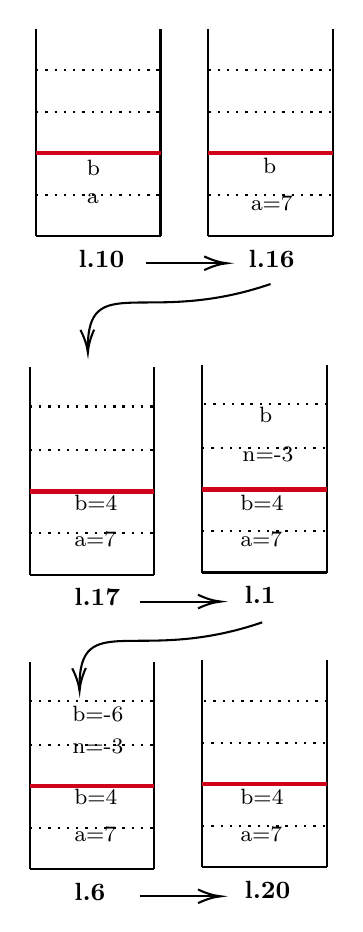
\begin{tikzpicture}[x=0.75pt,y=0.75pt,yscale=-1,xscale=1]
%uncomment if require: \path (0,458); %set diagram left start at 0, and has height of 458

%Straight Lines [id:da8429734700510807] 
\draw    (30,23) -- (30,123) ;
%Straight Lines [id:da19831219285848856] 
\draw    (90,23) -- (90,123) ;
%Straight Lines [id:da5400213758858614] 
\draw    (30,123) -- (90,123) ;
%Straight Lines [id:da4614811810152353] 
\draw [color={rgb, 255:red, 208; green, 2; blue, 27 }  ,draw opacity=1 ][line width=1.5]    (30,83) -- (90,83) ;
%Straight Lines [id:da7418312957703486] 
\draw  [dash pattern={on 0.84pt off 2.51pt}]  (30,63) -- (90,63) ;
%Straight Lines [id:da44220893730007305] 
\draw  [dash pattern={on 0.84pt off 2.51pt}]  (30,43) -- (90,43) ;
%Straight Lines [id:da7122818634177301] 
\draw  [dash pattern={on 0.84pt off 2.51pt}]  (30,103) -- (90,103) ;
%Straight Lines [id:da8889841168006463] 
\draw    (113,23) -- (113,123) ;
%Straight Lines [id:da8250795297667006] 
\draw    (173,23) -- (173,123) ;
%Straight Lines [id:da153769027415249] 
\draw    (113,123) -- (173,123) ;
%Straight Lines [id:da3409745261003547] 
\draw [color={rgb, 255:red, 208; green, 2; blue, 27 }  ,draw opacity=1 ][line width=1.5]    (113,83) -- (173,83) ;
%Straight Lines [id:da30918279252694725] 
\draw  [dash pattern={on 0.84pt off 2.51pt}]  (113,63) -- (173,63) ;
%Straight Lines [id:da08149576778013312] 
\draw  [dash pattern={on 0.84pt off 2.51pt}]  (113,43) -- (173,43) ;
%Straight Lines [id:da9382181967763386] 
\draw  [dash pattern={on 0.84pt off 2.51pt}]  (113,103) -- (173,103) ;
%Straight Lines [id:da6241130854562982] 
\draw    (27,186) -- (27,286) ;
%Straight Lines [id:da0652329920065271] 
\draw    (87,186) -- (87,286) ;
%Straight Lines [id:da3427737768337946] 
\draw    (27,286) -- (87,286) ;
%Straight Lines [id:da6948639110517265] 
\draw [color={rgb, 255:red, 208; green, 2; blue, 27 }  ,draw opacity=1 ][line width=1.5]    (27,246) -- (87,246) ;
%Straight Lines [id:da10521662086391781] 
\draw  [dash pattern={on 0.84pt off 2.51pt}]  (27,226) -- (87,226) ;
%Straight Lines [id:da1799171590295756] 
\draw  [dash pattern={on 0.84pt off 2.51pt}]  (27,205) -- (87,205) ;
%Straight Lines [id:da8573807604872521] 
\draw  [dash pattern={on 0.84pt off 2.51pt}]  (27,266) -- (87,266) ;
%Straight Lines [id:da8546373787245809] 
\draw    (110,185) -- (110,285) ;
%Straight Lines [id:da5057514633946132] 
\draw    (170,185) -- (170,285) ;
%Straight Lines [id:da11330607845027241] 
\draw    (110,285) -- (170,285) ;
%Straight Lines [id:da5391591892099901] 
\draw [color={rgb, 255:red, 208; green, 2; blue, 27 }  ,draw opacity=1 ][line width=1.5]    (110,245) -- (170,245) ;
%Straight Lines [id:da4121209376162154] 
\draw  [dash pattern={on 0.84pt off 2.51pt}]  (110,225) -- (170,225) ;
%Straight Lines [id:da07063042445625389] 
\draw  [dash pattern={on 0.84pt off 2.51pt}]  (111,204) -- (171,204) ;
%Straight Lines [id:da31871463824678514] 
\draw  [dash pattern={on 0.84pt off 2.51pt}]  (110,265) -- (170,265) ;
%Straight Lines [id:da8736620559119563] 
\draw    (83,136) -- (120,136) ;
\draw [shift={(122,136)}, rotate = 180] [color={rgb, 255:red, 0; green, 0; blue, 0 }  ][line width=0.75]    (10.93,-3.29) .. controls (6.95,-1.4) and (3.31,-0.3) .. (0,0) .. controls (3.31,0.3) and (6.95,1.4) .. (10.93,3.29)   ;
%Straight Lines [id:da4332825975230299] 
\draw    (80,299) -- (117,299) ;
\draw [shift={(119,299)}, rotate = 180] [color={rgb, 255:red, 0; green, 0; blue, 0 }  ][line width=0.75]    (10.93,-3.29) .. controls (6.95,-1.4) and (3.31,-0.3) .. (0,0) .. controls (3.31,0.3) and (6.95,1.4) .. (10.93,3.29)   ;
%Curve Lines [id:da3541341893057093] 
\draw    (143,146) .. controls (82.91,166.69) and (54.85,138.86) .. (54.97,177.2) ;
\draw [shift={(55,179)}, rotate = 268.6] [color={rgb, 255:red, 0; green, 0; blue, 0 }  ][line width=0.75]    (10.93,-3.29) .. controls (6.95,-1.4) and (3.31,-0.3) .. (0,0) .. controls (3.31,0.3) and (6.95,1.4) .. (10.93,3.29)   ;
%Straight Lines [id:da3937643351432618] 
\draw    (27,328) -- (27,428) ;
%Straight Lines [id:da8597551176172733] 
\draw    (87,328) -- (87,428) ;
%Straight Lines [id:da38963006223596564] 
\draw    (27,428) -- (87,428) ;
%Straight Lines [id:da5412618169618728] 
\draw [color={rgb, 255:red, 208; green, 2; blue, 27 }  ,draw opacity=1 ][line width=1.5]    (27,388) -- (87,388) ;
%Straight Lines [id:da03877447581091542] 
\draw  [dash pattern={on 0.84pt off 2.51pt}]  (27,368) -- (87,368) ;
%Straight Lines [id:da4010739204563538] 
\draw  [dash pattern={on 0.84pt off 2.51pt}]  (27,347) -- (87,347) ;
%Straight Lines [id:da12294595698868216] 
\draw  [dash pattern={on 0.84pt off 2.51pt}]  (27,408) -- (87,408) ;
%Straight Lines [id:da169589200405734] 
\draw    (110,327) -- (110,427) ;
%Straight Lines [id:da9183842982319133] 
\draw    (170,327) -- (170,427) ;
%Straight Lines [id:da598862808777054] 
\draw    (110,427) -- (170,427) ;
%Straight Lines [id:da9776105886381585] 
\draw [color={rgb, 255:red, 208; green, 2; blue, 27 }  ,draw opacity=1 ][line width=1.5]    (110,387) -- (170,387) ;
%Straight Lines [id:da8693644383109624] 
\draw  [dash pattern={on 0.84pt off 2.51pt}]  (110,407) -- (170,407) ;
%Straight Lines [id:da9626408520035064] 
\draw    (80,441) -- (117,441) ;
\draw [shift={(119,441)}, rotate = 180] [color={rgb, 255:red, 0; green, 0; blue, 0 }  ][line width=0.75]    (10.93,-3.29) .. controls (6.95,-1.4) and (3.31,-0.3) .. (0,0) .. controls (3.31,0.3) and (6.95,1.4) .. (10.93,3.29)   ;
%Curve Lines [id:da11800089051451801] 
\draw    (139,309) .. controls (78.91,329.69) and (50.85,301.86) .. (50.97,340.2) ;
\draw [shift={(51,342)}, rotate = 268.6] [color={rgb, 255:red, 0; green, 0; blue, 0 }  ][line width=0.75]    (10.93,-3.29) .. controls (6.95,-1.4) and (3.31,-0.3) .. (0,0) .. controls (3.31,0.3) and (6.95,1.4) .. (10.93,3.29)   ;
%Straight Lines [id:da027673471348472978] 
\draw  [dash pattern={on 0.84pt off 2.51pt}]  (111,347) -- (171,347) ;
%Straight Lines [id:da3914465095869988] 
\draw  [dash pattern={on 0.84pt off 2.51pt}]  (110,367) -- (170,367) ;

% Text Node
\draw (49,128) node [anchor=north west][inner sep=0.75pt]   [align=left] {\textbf{{\small l.10}}};
% Text Node
\draw (131,128) node [anchor=north west][inner sep=0.75pt]   [align=left] {\textbf{{\small l.16}}};
% Text Node
\draw (47,291) node [anchor=north west][inner sep=0.75pt]   [align=left] {\textbf{{\small l.17}}};
% Text Node
\draw (129,290) node [anchor=north west][inner sep=0.75pt]   [align=left] {\textbf{{\small l.1}}};
% Text Node
\draw (53,101) node [anchor=north west][inner sep=0.75pt]   [align=left] {{\footnotesize a}};
% Text Node
\draw (53,85) node [anchor=north west][inner sep=0.75pt]   [align=left] {{\footnotesize b}};
% Text Node
\draw (132,102) node [anchor=north west][inner sep=0.75pt]   [align=left] {{\footnotesize a=7}};
% Text Node
\draw (138,84) node [anchor=north west][inner sep=0.75pt]   [align=left] {{\footnotesize b}};
% Text Node
\draw (47,264) node [anchor=north west][inner sep=0.75pt]   [align=left] {{\footnotesize a=7}};
% Text Node
\draw (47,246) node [anchor=north west][inner sep=0.75pt]   [align=left] {{\footnotesize b=4}};
% Text Node
\draw (127,264) node [anchor=north west][inner sep=0.75pt]   [align=left] {{\footnotesize a=7}};
% Text Node
\draw (127,246) node [anchor=north west][inner sep=0.75pt]   [align=left] {{\footnotesize b=4}};
% Text Node
\draw (128,223) node [anchor=north west][inner sep=0.75pt]   [align=left] {{\footnotesize n=-3}};
% Text Node
\draw (136,204) node [anchor=north west][inner sep=0.75pt]   [align=left] {{\footnotesize b}};
% Text Node
\draw (47,433) node [anchor=north west][inner sep=0.75pt]   [align=left] {\textbf{{\small l.6}}};
% Text Node
\draw (129,432) node [anchor=north west][inner sep=0.75pt]   [align=left] {\textbf{{\small l.20}}};
% Text Node
\draw (47,406) node [anchor=north west][inner sep=0.75pt]   [align=left] {{\footnotesize a=7}};
% Text Node
\draw (47,388) node [anchor=north west][inner sep=0.75pt]   [align=left] {{\footnotesize b=4}};
% Text Node
\draw (127,406) node [anchor=north west][inner sep=0.75pt]   [align=left] {{\footnotesize a=7}};
% Text Node
\draw (127,388) node [anchor=north west][inner sep=0.75pt]   [align=left] {{\footnotesize b=4}};
% Text Node
\draw (46,364) node [anchor=north west][inner sep=0.75pt]   [align=left] {{\footnotesize n=-3}};
% Text Node
\draw (46,348) node [anchor=north west][inner sep=0.75pt]   [align=left] {{\footnotesize b=-6}};


\end{tikzpicture}

\end{minipage}
\textbf{\pasapas Explications}\\
Lors de l'exécution d'une fonction, avant même la lecture des instructions, le processeur alloue un espace mémoire pour chacune des variables déclarées. Par ailleurs, les arguments des fonctions sont \textbf{passés par valeurs}. Ce faisant, une copie locale de ceux-si sont effectués. Ensuite, lignes par lignes, les différentes instructions sont traitées, avec entre autre les différentes initialisations. Lorsque l'exécution de la fonction secondaire s'achève, les variables sont dépilées. 

\subsubsection{Les fonctions}
Une fonction est une factorisation du programme, qui peut-être exploitée dans l'ensemble de celui-ci. 
\subsubsubsection{Définition}
La définition d'une fonction suit la syntaxe suivante:
\begin{minted}{c}
type identificateur(type arg1,..., type argn){

    [declaration de variables locales]

    corps de la fonction

}
\end{minted}
\begin{itemize}
    \flch \mintinline{c}{type} est le type de retour de la fonction. En conséquence de quoi, le corps de la fonction fait mention d'une ou plusieurs instructions \mintinline{c}{return expression;} où \mintinline{c}{expression} est de type \mintinline{c}{type}.
    \flch \mintinline{c}{identificateur} suit les règles de construction mentionnée dans la sous-section \textcolor{doubleu}{\nameref{ident}}
    \flch Est encapsulée l'énumération des arguments, ici appelés \textbf{paramètres formels}, précédés de leurs types. Si la fonction ne prend pas de paramètres, on écrira \mintinline{c}{() ou (void)}
\end{itemize}
De plus, une fonction peut s'appeler au sein d'elle-même, c'est ce que l'on appelle la récursivité; et faire appel à d'autres fonctions. Toutefois, à l'instar du OCaml par exemple, il est impossible de définir des fonctions auxiliaires dans le corps même d'une fonction.
\begin{code}
    Tout programme contient au moins une fonction, en C, c'est la fonction \mintinline{c}{main} qui à le prototype suivant: \mintinline{c}{int main(int argc, char* argv)} ou dans des cas d'utilisation plus basique \mintinline{c}{int main(void)}.
\end{code}
\subsubsubsection{Déclaration}
Toutefois, pour que le compilateur soit au fait de l'existence de telle ou telle fonction, il est nécessaire qu'avant chaque appel, elle ait été déclarée. Pour se faire, il faut mentionner le prototype de chacune des fonctions du programme avant tout appel à celle-ci. La déclaration suit la syntaxe suivante:
\begin{minted}{c}
type identificateur(type_1 arg1,..., type_n argn);
\end{minted}
\begin{rem}{0}
    On se référera à la section XXX pour comprendre quand et où la déclaration des fonctions s'avère nécessaire.
\end{rem} 
\subsubsubsection{Appel}
L'appel à une fonction suit la syntaxe suivante:
\begin{center}
\mintinline{c}{identificateur(arg1,...,argn);}
\end{center}
Les arguments donnés à la fonction constituent les \textbf{paramètres effectifs} et doivent concorder avec la définition de la fonction. 
\begin{code}
    Les paramètres effectifs sont \textbf{passés par valeurs} lors de l'exécution de la fonction. Ce faisant, le compilateur réalise une copie locale à la fonction des arguments et les ajoute dans pile. Par conséquent, il est important de comprendre qu'en fournissant seulement la valeur des arguments, les fonctions ne sont pas en mesure de les modifier à l'extérieur de celle-ci. On verra par la suite pour qu'opérer de façon effective sur des variables extérieure à la fonction, il est nécessaire de \textbf{passer par référence} les arguments. (XXX)
\end{code}
\subsubsubsection{Compléments}
\vspace*{-0.5cm}
\begin{itemize}
    \flch \textbf{La fonction main}
    \flch \textbf{Fonction à paramètres variables}
\end{itemize}
\subsubsection{Structures conditionnelles}
\subsubsubsection{L'alternative}
L'alternative est une structure de contrôle conditionnelles en ce qu'elle permet l'exécution d'un certain nombre d'instructions si et seulement si une expression booléenne est vérifiée. 
\begin{minted}{c}
    if(cond){
        // Corps du if
    }
    else{
        // Corps du else
    }
\end{minted}
\begin{rem}{0}
    Il n'est pas nécessaire qu'il y ait un \mintinline{c}{else}. 
\end{rem}
\subsubsubsection{Opérateur ternaire}
\begin{center}
    \mintinline{c}{condition ? expression : expression}
\end{center}
L'opérateur conditionnel (?:) requiert trois opérandes
\begin{itemize}
    \flch une condition qui est une expression logique convertie en \mintinline{c}{bool}
    \flch deux expressions résultantes
\end{itemize}
Si la condition est évaluée à \mintinline{c}{true}, alors la première expression est évaluée. Sinon, la seconde est évaluée.\\[0.5cm]
\textbf{Exemple}\\
\vspace*{-0.5cm}
\begin{minted}{c}
    int main(){
        int i;
        scanf("%d",&i); // Saisie de i par l'utilisateur
        
        int j=i%2?i/2:(i+1)/2;
        
        return 0;
    }
\end{minted}
Ici l'opérateur \% correspond à l'opérateur de la congruence. En l'occurrence, si l'utilisateur à saisi une valeur paire pour i, alors j apprend $\frac{i}{2}$ sinon $\frac{i+1}{2}$. (Ici, $j\=\lceil\frac{i}{2}\rceil$)
\begin{rem}{0.5}
    Cet opérateur est peu utilisé compte-tenu de son manque de lisibilité. 
\end{rem}
\subsubsubsection{Le branchement multiple}
L'objectif du branchement multiple et de s'épargner une répétition de \mintinline{c}{if(expression==x)} ou x admet des valeurs dans un ensemble fini de taille relativement faible et défini explicitement. Ce faisant, il s'agit de "matcher" l'expression avec ses différentes possibilités. Dans le cas ou l'expression ne correspond à aucun des cas énumérés, alors ce sont les instructions contenues dans \mintinline{c}{default} qui sont exécutés. 
\begin{minted}{c}
switch(expression){
    case exp:
        // Cas 1
    break;
    ...
    case exp:
        // Cas n
    break;
    default:
        // Cas de défaut
    break;
}
\end{minted}
\begin{rem}{0}
    Il n'est pas nécessaire de faire figurer une alternative \mintinline{c}{default}.\\
    Le mot-clé \mintinline{c}{break} permet de sortir du dernier corps \{\}.
\end{rem}
\subsubsection{Les boucles}
\subsubsubsection{Tant que...}
\begin{minted}{c}
while(condition){
    // Corps de boucle 
}
\end{minted}
\subsubsubsection{Pour ...}
\begin{minted}{c}
for(valeur initiale;valeur finale;incrémentation){
    // Corps de boucle
}
\end{minted}
\subsubsubsection{Faire ... Tant que}
\begin{minted}{c}
do{
    // Corprs de boucle
}while(condition);
\end{minted}
Fonctionnement similaire à une boucle while, à la différence qu'au moins un tout de boucle est réalisé.
\subsubsubsection{Passes-droit}
Il est possible de mettre un terme à l'exécution d'une boucle, et en cas de boucle imbriquée de sortir de la boucle la plus interne, à l'aide du mot-clé: \mintinline{c}{break;}\\[0.5cm]
Étant donnée une étiquette, \ie un mot-clé inscrit à un endroit du code, d'effectuer un saut dans le programme à l'endroit indiqué par l'étiquette par le biais de l'instruction \mintinline{c}{goto étiquette}.
\begin{code}
Une telle instruction \mintinline{c}{goto} est à proscrire.\hfill\dangersign[4ex]
\end{code}